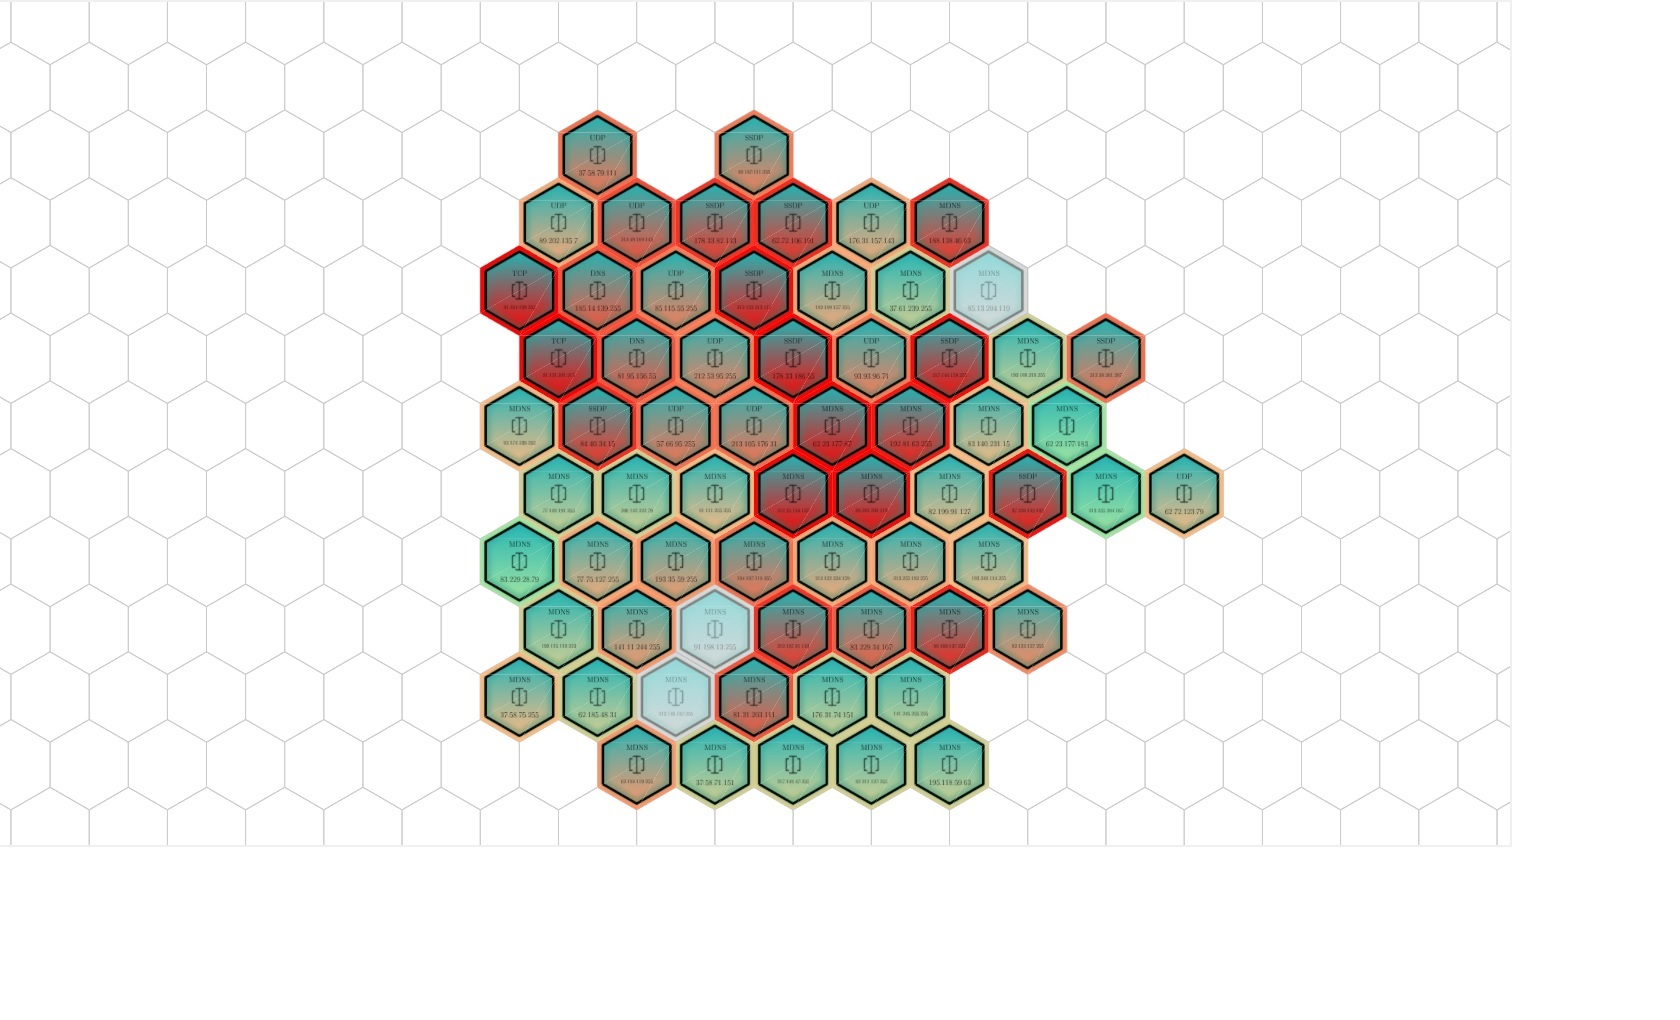
\includegraphics[width=\linewidth]{materials/heat-map.jpg}
The Heat Map visualization uses a hexagonal map to display a compacty cluster of nodes.
Each machine found to be communicating in the analysed network will be represented as a node.
The activity of a specific machine in the network is represented by the colour of the 
corresponding hexagon. As more and more traffic arises, nodes representing the machines that
send and reveive data ``heat up'' and, as the time passes, ``cool down''.
The hexagonal grid is being filled in a compact manner - new nodes are place outside of 
the already displayed nodes. The relative position of the map elements in this visualization
does not play a role on default. There is a way to sort the nodes so that they form a radial 
gradient - the more ``heated up'' will be sorted to the middle.

This visualization helps a user find machines that are most active in the network.
It gives a quick overview of the number of the clients and how many of them are currently active.
Additionaly every node presents some information, such as the machine's most commonly used protocol.
This lets users do some basic data selection choices easily. For example: if some other visualization
is being obscured by too much data from one specific machine, or too much data of some protocol,
the user can look at the heatmap and find out what filters to apply to make the overview of the situation
more clear.
